\documentclass{standalone}[9pt]
% main document, called main.tex
\usepackage{tikz}
\usetikzlibrary{external}
\tikzexternalize % activate!
\begin{document}

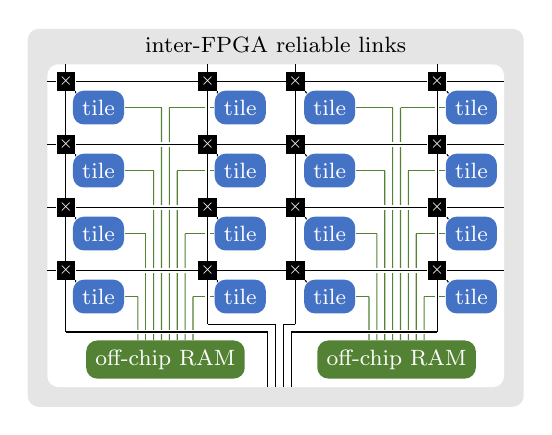
\begin{tikzpicture}
  [scale=.5,auto=left,every node/.style={rectangle
    ,fill=myblue,text=white},align=center]
  \definecolor{myblue}{RGB}{68,114,196}
  \definecolor{myorange}{RGB}{197,90,17}
  \definecolor{myorange}{RGB}{197,90,17}
  \definecolor{mygreen}{RGB}{84,130,53}

  \node[fill=gray!20,rounded corners,
        minimum width=6.3cm,minimum height=4.8cm] (border0)
    at (4.5,2.0) {};
  \node[fill=white,rounded corners,
        minimum width=5.8cm,minimum height=4.1cm] (border1)
    at (4.5,1.8) {};
  \node[fill=none,color=black] at (4.5,6.4)
    {\footnotesize{inter-FPGA reliable links}};

  \node[fill=myblue,rounded corners] (tile00)
     at (0,0) {\footnotesize{tile}};
  \node[rectangle,sharp corners,fill=black] (router00)
     at (-0.83,0.664) {};
  \node[fill=none] (x00)
     at (-0.83,0.664) {\tiny{$\times$}};
  \draw[arrows=-,color=black] (router00.south east) to
    ([xshift=0.8mm,yshift=-0.8mm]tile00.north west);

  \node[fill=myblue,rounded corners] (tile01)
     at (0,1.6) {\footnotesize{tile}};
  \node[rectangle,sharp corners,fill=black] (router01)
     at (-0.83,2.264) {};
  \node[fill=none] (x01)
     at (-0.83,2.264) {\tiny{$\times$}};
  \draw[arrows=-,color=black] (router01.south east) to
    ([xshift=0.8mm,yshift=-0.8mm]tile01.north west);

  \node[fill=myblue,rounded corners] (tile02)
     at (0,3.2) {\footnotesize{tile}};
  \node[rectangle,sharp corners,fill=black] (router02)
     at (-0.83,3.864) {};
  \node[fill=none] (x02)
     at (-0.83,3.864) {\tiny{$\times$}};
  \draw[arrows=-,color=black] (router02.south east) to
    ([xshift=0.8mm,yshift=-0.8mm]tile02.north west);

  \node[fill=myblue,rounded corners] (tile03)
     at (0,4.8) {\footnotesize{tile}};
  \node[rectangle,sharp corners,fill=black] (router03)
     at (-0.83,5.464) {};
  \node[fill=none] (x03)
     at (-0.83,5.464) {\tiny{$\times$}};
  \draw[arrows=-,color=black] (router03.south east) to
    ([xshift=0.8mm,yshift=-0.8mm]tile03.north west);


  \node[fill=myblue,rounded corners] (tile10)
     at (3.6,0) {\footnotesize{tile}};
  \node[rectangle,sharp corners,fill=black] (router10)
     at (2.77,0.664) {};
  \node[fill=none] (x10)
     at (2.77,0.664) {\tiny{$\times$}};
  \draw[arrows=-,color=black] (router10.south east) to
    ([xshift=0.8mm,yshift=-0.8mm]tile10.north west);

  \node[fill=myblue,rounded corners] (tile11)
     at (3.6,1.6) {\footnotesize{tile}};
  \node[rectangle,sharp corners,fill=black] (router11)
     at (2.77,2.264) {};
  \node[fill=none] (x11)
     at (2.77,2.264) {\tiny{$\times$}};
  \draw[arrows=-,color=black] (router11.south east) to
    ([xshift=0.8mm,yshift=-0.8mm]tile11.north west);

  \node[fill=myblue,rounded corners] (tile12)
     at (3.6,3.2) {\footnotesize{tile}};
  \node[rectangle,sharp corners,fill=black] (router12)
     at (2.77,3.864) {};
  \node[fill=none] (x12)
     at (2.77,3.864) {\tiny{$\times$}};
  \draw[arrows=-,color=black] (router12.south east) to
    ([xshift=0.8mm,yshift=-0.8mm]tile12.north west);

  \node[fill=myblue,rounded corners] (tile13)
     at (3.6,4.8) {\footnotesize{tile}};
  \node[rectangle,sharp corners,fill=black] (router13)
     at (2.77,5.464) {};
  \node[fill=none] (x13)
     at (2.77,5.464) {\tiny{$\times$}};
  \draw[arrows=-,color=black] (router13.south east) to
    ([xshift=0.8mm,yshift=-0.8mm]tile13.north west);



  \coordinate[] (mem00) at (1,0) {};
  \draw[arrows=-,color=mygreen] (tile00) to (mem00);

  \coordinate[] (mem01) at (1.2,1.6) {};
  \draw[arrows=-,color=mygreen] (tile01) to (mem01);

  \coordinate[] (mem02) at (1.4,3.2) {};
  \draw[arrows=-,color=mygreen] (tile02) to (mem02);

  \coordinate[] (mem03) at (1.6,4.8) {};
  \draw[arrows=-,color=mygreen] (tile03) to (mem03);

  \coordinate[] (mem10) at (2.4,0) {};
  \draw[arrows=-,color=mygreen] (tile10) to (mem10);

  \coordinate[] (mem11) at (2.2,1.6) {};
  \draw[arrows=-,color=mygreen] (tile11) to (mem11);

  \coordinate[] (mem12) at (2.0,3.2) {};
  \draw[arrows=-,color=mygreen] (tile12) to (mem12);

  \coordinate[] (mem13) at (1.8,4.8) {};
  \draw[arrows=-,color=mygreen] (tile13) to (mem13);

  \node[rounded corners,fill=mygreen]
    (ram0) at (1.7,-1.6) {\footnotesize{off-chip RAM}};

  \draw[arrows=-,color=mygreen] (mem00) to ([xshift=-7mm]ram0.north);
  \draw[arrows=-,color=mygreen] (mem01) to ([xshift=-5mm]ram0.north);
  \draw[arrows=-,color=mygreen] (mem02) to ([xshift=-3mm]ram0.north);
  \draw[arrows=-,color=mygreen] (mem03) to ([xshift=-1mm]ram0.north);
  \draw[arrows=-,color=mygreen] (mem10) to ([xshift=7mm]ram0.north);
  \draw[arrows=-,color=mygreen] (mem11) to ([xshift=5mm]ram0.north);
  \draw[arrows=-,color=mygreen] (mem12) to ([xshift=3mm]ram0.north);
  \draw[arrows=-,color=mygreen] (mem13) to ([xshift=1mm]ram0.north);

  \coordinate[] (south0b) at (4.3, -0.9) {};
  \coordinate[] (south0a) at (-0.83, -0.9) {};
  \draw[arrows=-,color=white,line width=0.6mm] (south0a) to (south0b);
  \draw[arrows=-,color=black] (router00.south) to (south0a);
  \draw[arrows=-,color=black] (south0a) to (south0b);
  \coordinate[] (south0c) at (4.3, -2.3) {};
  \draw[arrows=-,color=black] (south0b) to (south0c);

  \coordinate[] (south1a) at (2.77, -0.7) {};
  \draw[arrows=-,color=white,line width=0.6mm] (router10.south) to (south1a);
  \draw[arrows=-,color=black] (router10.south) to (south1a);
  \coordinate[] (south1b) at (4.5, -0.7) {};
  \draw[arrows=-,color=black] (south1a) to (south1b);
  \coordinate[] (south1c) at (4.5, -2.3) {};
  \draw[arrows=-,color=black] (south1b) to (south1c);
  
  \draw[arrows=-,color=black] (router00.north) to (router01.south);
  \draw[arrows=-,color=black] (router01.north) to (router02.south);
  \draw[arrows=-,color=black] (router02.north) to (router03.south);

  \draw[arrows=-,color=white,line width=0.6mm]
    (router00.east) to (router10.west);
  \draw[arrows=-,color=black] (router00.east) to (router10.west);

  \draw[arrows=-,color=white,line width=0.6mm]
    (router01.east) to (router11.west);
  \draw[arrows=-,color=black] (router01.east) to (router11.west);

  \draw[arrows=-,color=white,line width=0.6mm]
    (router02.east) to (router12.west);
  \draw[arrows=-,color=black] (router02.east) to (router12.west);

  \draw[arrows=-,color=black] (router03.east) to (router13.west);

  \draw[arrows=-,color=white,line width=0.6mm]
    (router10.north) to (router11.south);
  \draw[arrows=-,color=black] (router10.north) to (router11.south);

  \draw[arrows=-,color=white,line width=0.6mm]
    (router11.north) to (router12.south);
  \draw[arrows=-,color=black] (router11.north) to (router12.south);

  \draw[arrows=-,color=white,line width=0.6mm]
    (router12.north) to (router13.south);
  \draw[arrows=-,color=black] (router12.north) to (router13.south);

  %%%

  \node[fill=myblue,rounded corners] (tile20)
     at (5.87,0) {\footnotesize{tile}};
  \node[rectangle,sharp corners,fill=black] (router20)
     at (5,0.664) {};
  \node[fill=none] (x20)
     at (5,0.664) {\tiny{$\times$}};
  \draw[arrows=-,color=black] (router20.south east) to
    ([xshift=0.8mm,yshift=-0.8mm]tile20.north west);

  \node[fill=myblue,rounded corners] (tile21)
     at (5.87,1.6) {\footnotesize{tile}};
  \node[rectangle,sharp corners,fill=black] (router21)
     at (5,2.264) {};
  \node[fill=none] (x21)
     at (5,2.264) {\tiny{$\times$}};
  \draw[arrows=-,color=black] (router21.south east) to
    ([xshift=0.8mm,yshift=-0.8mm]tile21.north west);

  \node[fill=myblue,rounded corners] (tile22)
     at (5.87,3.2) {\footnotesize{tile}};
  \node[rectangle,sharp corners,fill=black] (router22)
     at (5,3.864) {};
  \node[fill=none] (x22)
     at (5,3.864) {\tiny{$\times$}};
  \draw[arrows=-,color=black] (router22.south east) to
    ([xshift=0.8mm,yshift=-0.8mm]tile22.north west);

  \node[fill=myblue,rounded corners] (tile23)
     at (5.87,4.8) {\footnotesize{tile}};
  \node[rectangle,sharp corners,fill=black] (router23)
     at (5,5.464) {};
  \node[fill=none] (x23)
     at (5,5.464) {\tiny{$\times$}};
  \draw[arrows=-,color=black] (router23.south east) to
    ([xshift=0.8mm,yshift=-0.8mm]tile23.north west);



  \node[fill=myblue,rounded corners] (tile30)
     at (9.47,0) {\footnotesize{tile}};
  \node[rectangle,sharp corners,fill=black] (router30)
     at (8.6,0.664) {};
  \node[fill=none] (x30)
     at (8.6,0.664) {\tiny{$\times$}};
  \draw[arrows=-,color=black] (router30.south east) to
    ([xshift=0.8mm,yshift=-0.8mm]tile30.north west);

  \node[fill=myblue,rounded corners] (tile31)
     at (9.47,1.6) {\footnotesize{tile}};
  \node[rectangle,sharp corners,fill=black] (router31)
     at (8.6,2.264) {};
  \node[fill=none] (x31)
     at (8.6,2.264) {\tiny{$\times$}};
  \draw[arrows=-,color=black] (router31.south east) to
    ([xshift=0.8mm,yshift=-0.8mm]tile31.north west);

  \node[fill=myblue,rounded corners] (tile32)
     at (9.47,3.2) {\footnotesize{tile}};
  \node[rectangle,sharp corners,fill=black] (router32)
     at (8.6,3.864) {};
  \node[fill=none] (x32)
     at (8.6,3.864) {\tiny{$\times$}};
  \draw[arrows=-,color=black] (router32.south east) to
    ([xshift=0.8mm,yshift=-0.8mm]tile32.north west);

  \node[fill=myblue,rounded corners] (tile33)
     at (9.47,4.8) {\footnotesize{tile}};
  \node[rectangle,sharp corners,fill=black] (router33)
     at (8.6,5.464) {};
  \node[fill=none] (x13)
     at (8.6,5.464) {\tiny{$\times$}};
  \draw[arrows=-,color=black] (router33.south east) to
    ([xshift=0.8mm,yshift=-0.8mm]tile33.north west);


  \coordinate[] (memb00) at (6.87,0) {};
  \draw[arrows=-,color=mygreen] (tile20) to (memb00);

  \coordinate[] (memb01) at (7.07,1.6) {};
  \draw[arrows=-,color=mygreen] (tile21) to (memb01);

  \coordinate[] (memb02) at (7.27,3.2) {};
  \draw[arrows=-,color=mygreen] (tile22) to (memb02);

  \coordinate[] (memb03) at (7.47,4.8) {};
  \draw[arrows=-,color=mygreen] (tile23) to (memb03);

  \coordinate[] (memb10) at (8.27,0) {};
  \draw[arrows=-,color=mygreen] (tile30) to (memb10);

  \coordinate[] (memb11) at (8.07,1.6) {};
  \draw[arrows=-,color=mygreen] (tile31) to (memb11);

  \coordinate[] (memb12) at (7.87,3.2) {};
  \draw[arrows=-,color=mygreen] (tile32) to (memb12);

  \coordinate[] (memb13) at (7.67,4.8) {};
  \draw[arrows=-,color=mygreen] (tile33) to (memb13);

  \node[rounded corners,fill=mygreen]
    (ram1) at (7.57,-1.6) {\footnotesize{off-chip RAM}};

  \draw[arrows=-,color=mygreen] (memb00) to ([xshift=-7mm]ram1.north);
  \draw[arrows=-,color=mygreen] (memb01) to ([xshift=-5mm]ram1.north);
  \draw[arrows=-,color=mygreen] (memb02) to ([xshift=-3mm]ram1.north);
  \draw[arrows=-,color=mygreen] (memb03) to ([xshift=-1mm]ram1.north);
  \draw[arrows=-,color=mygreen] (memb10) to ([xshift=7mm]ram1.north);
  \draw[arrows=-,color=mygreen] (memb11) to ([xshift=5mm]ram1.north);
  \draw[arrows=-,color=mygreen] (memb12) to ([xshift=3mm]ram1.north);
  \draw[arrows=-,color=mygreen] (memb13) to ([xshift=1mm]ram1.north);





  \draw[arrows=-,color=white,line width=0.6mm]
    (router20.east) to (router30.west);
  \draw[arrows=-,color=black] (router20.east) to (router30.west);
  \draw[arrows=-,color=white,line width=0.6mm]
    (router21.east) to (router31.west);
  \draw[arrows=-,color=black] (router21.east) to (router31.west);
  \draw[arrows=-,color=white,line width=0.6mm]
    (router22.east) to (router32.west);
  \draw[arrows=-,color=black] (router22.east) to (router32.west);
  \draw[arrows=-,color=white,line width=0.6mm]
    (router23.east) to (router33.west);
  \draw[arrows=-,color=black] (router23.east) to (router33.west);

  \draw[arrows=-,color=white,line width=0.6mm]
    (router10.east) to (router20.west);
  \draw[arrows=-,color=black] (router10.east) to (router20.west);
  \draw[arrows=-,color=white,line width=0.6mm]
    (router11.east) to (router21.west);
  \draw[arrows=-,color=black] (router11.east) to (router21.west);
  \draw[arrows=-,color=white,line width=0.6mm]
    (router12.east) to (router22.west);
  \draw[arrows=-,color=black] (router12.east) to (router22.west);
  \draw[arrows=-,color=white,line width=0.6mm]
    (router13.east) to (router23.west);
  \draw[arrows=-,color=black] (router13.east) to (router23.west);

  \draw[arrows=-,color=white,line width=0.6mm]
    (router20.north) to (router21.south);
  \draw[arrows=-,color=black] (router20.north) to (router21.south);
  \draw[arrows=-,color=white,line width=0.6mm]
    (router21.north) to (router22.south);
  \draw[arrows=-,color=black] (router21.north) to (router22.south);
  \draw[arrows=-,color=white,line width=0.6mm]
    (router22.north) to (router23.south);
  \draw[arrows=-,color=black] (router22.north) to (router23.south);

  \draw[arrows=-,color=white,line width=0.6mm]
    (router30.north) to (router31.south);
  \draw[arrows=-,color=black] (router30.north) to (router31.south);
  \draw[arrows=-,color=white,line width=0.6mm]
    (router31.north) to (router32.south);
  \draw[arrows=-,color=black] (router31.north) to (router32.south);
  \draw[arrows=-,color=white,line width=0.6mm]
    (router32.north) to (router33.south);
  \draw[arrows=-,color=black] (router32.north) to (router33.south);

  \coordinate[] (south1a) at (8.6, -0.9) {};
  \coordinate[] (south1b) at (4.9, -0.9) {};
  \draw[arrows=-,color=white,line width=0.6mm] (router30.south) to (south1a);
  \draw[arrows=-,color=white,line width=0.6mm] (south1a) to (south1b);
  \draw[arrows=-,color=black] (router30.south) to (south1a);
  \draw[arrows=-,color=black] (south1a) to (south1b);
  \coordinate[] (south1c) at (4.9, -2.3) {};
  \draw[arrows=-,color=black] (south1b) to (south1c);

  \coordinate[] (south2a) at (5, -0.7) {};
  \draw[arrows=-,color=black] (router20.south) to (south2a);
  \coordinate[] (south2b) at (4.7, -0.7) {};
  \draw[arrows=-,color=black] (south2a) to (south2b);
  \coordinate[] (south2c) at (4.7, -2.3) {};
  \draw[arrows=-,color=black] (south2b) to (south2c);

  \draw[arrows=-,color=black] (router00.west) to
    ([xshift=-2.3mm]router00.west);
  \draw[arrows=-,color=black] (router01.west) to
    ([xshift=-2.3mm]router01.west);
  \draw[arrows=-,color=black] (router02.west) to
    ([xshift=-2.3mm]router02.west);
  \draw[arrows=-,color=black] (router03.west) to
    ([xshift=-2.3mm]router03.west);

  \draw[arrows=-,color=black] (router30.east) to
    ([xshift=14.4mm]router30.east);
  \draw[arrows=-,color=black] (router31.east) to
    ([xshift=14.4mm]router31.east);
  \draw[arrows=-,color=black] (router32.east) to
    ([xshift=14.4mm]router32.east);
  \draw[arrows=-,color=black] (router33.east) to
    ([xshift=14.4mm]router33.east);

  \draw[arrows=-,color=black] (router03.north) to
    ([yshift=2mm]router03.north);
  \draw[arrows=-,color=black] (router13.north) to
    ([yshift=2mm]router13.north);
  \draw[arrows=-,color=black] (router23.north) to
    ([yshift=2mm]router23.north);
  \draw[arrows=-,color=black] (router33.north) to
    ([yshift=2mm]router33.north);

\end{tikzpicture}

\end{document}
